\section{The blur limits fine structure logarithmically}
\label{sec:loglaw}

\subsection{Smoothing removes fine structure exponentially}

The one-dimensional version of the mechanism is a short inequality.

\begin{lemma}[Smoothing--uncertainty, one dimension]
\label{lem:smoothing1d}
Let $f \in L^2(\mathbb{R})$ and let $u = f * N(0,\sigma^2)$ be its blur. With $\bar x = \sigma^2\|u'\|^2/\|u\|^2$, the mean squared wavenumber of the blurred function in units of $1/\sigma^2$,
\begin{equation}
\sigma^2\|u'\|^2 \leq \bar x\, e^{-\bar x}\,\|f\|^2 .
\label{eq:smoothing1d}
\end{equation}
Equality holds when $|\hat f|$ is concentrated at a single wavenumber.
\end{lemma}

\begin{proof}
By Parseval, with $x = \sigma^2\xi^2$ and the probability measure $\nu \propto |\hat f(\xi)|^2 d\xi$, $\|u\|^2 = A\|f\|^2$ with $A = \int e^{-x}\,d\nu$, and $\sigma^2\|u'\|^2 = \|f\|^2\int x e^{-x}\,d\nu = \bar x A \|f\|^2$. Under $\mu = e^{-x}\nu/A$, Jensen's inequality gives $1/A = \E_\mu[e^x] \geq e^{\E_\mu x} = e^{\bar x}$.
\end{proof}

A structure that still looks fine after the blur ($\bar x$ large) can carry only a fraction $\bar x e^{-\bar x}$ of its original size as sharpness. Fine structure is not forbidden, but it is exponentially expensive. Figure~\ref{fig:lemma}a checks Eq.~\eqref{eq:smoothing1d} on 400 random structures (largest ratio $0.9992$); Fig.~\ref{fig:lemma}b shows that the windows of the strips follow the same law.

\begin{figure*}[t]
\centering
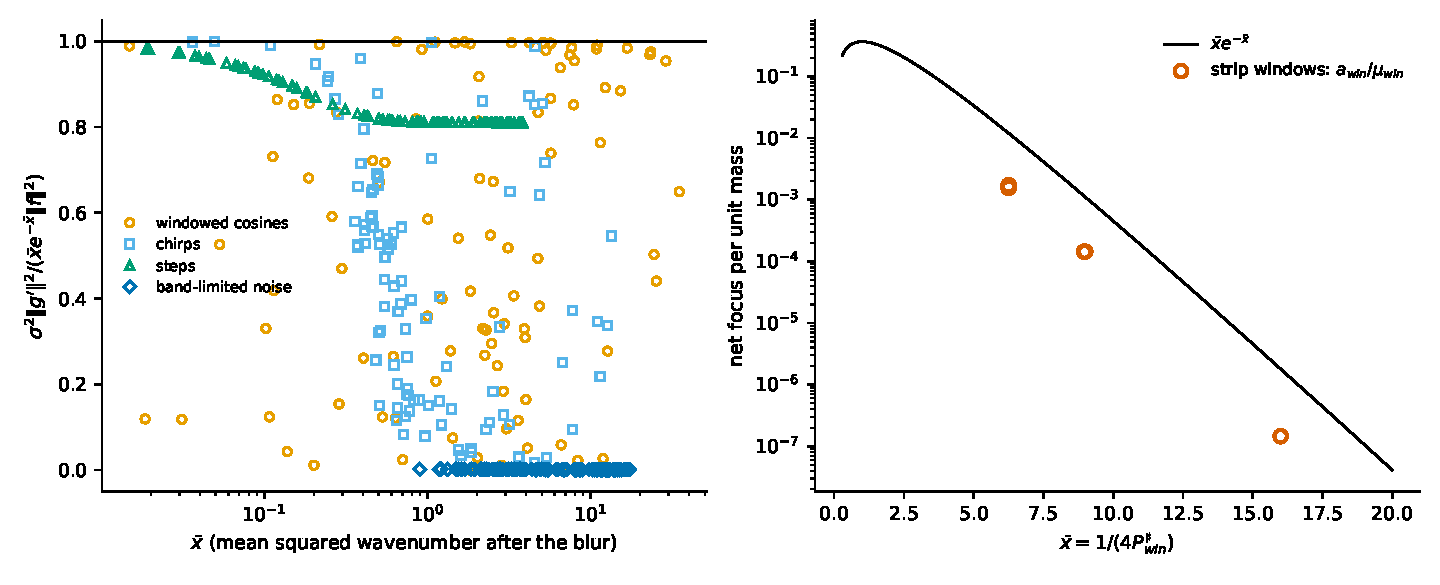
\includegraphics[width=0.85\textwidth]{figures/fig4_lemma.pdf}
\caption{(a) Lemma~\ref{lem:smoothing1d} on random one-dimensional structures: the ratio of the two sides of Eq.~\eqref{eq:smoothing1d} never exceeds one, and approaches one for a single wavenumber. (b) Sharpness per unit mass of the windows of the strips against $\bar x e^{-\bar x}$, with $\bar x$ taken from the window's spread (observed, not proved).}
\label{fig:lemma}
\end{figure*}

In the plane we apply the same argument to the part of the density that varies along the stable direction, with one refinement: we split the blur into two parts, use the first to remove fine structure and keep the second to compare norms. The confinement of the state then provides the floor.

\begin{lemma}[Split smoothing--uncertainty]
\label{lem:split}
Under (H1), for every $t \in (0,1)$,
\begin{equation}
\xb(\varrho) \leq \frac{1}{t}\Big[2\ln\frac1\sigma + \ln\frac{8(\pi^2 + \sigma^2/2)}{e\,t(1-t)}\Big].
\label{eq:split}
\end{equation}
Without (H1) the same holds with $\pi^2 + \sigma^2/2$ replaced by the state's own $\E_Q[y_z^2]$.
\end{lemma}

The proof (Appendix~\ref{app:split}) has four steps. Write $\varrho$ as a blur of variance $t\sigma^2$ of the partly blurred state $\rho * N(0,(1-t)\sigma^2)$. (i)~Jensen's inequality, as in Lemma~\ref{lem:smoothing1d}, shows that the second blur reduces $\|\partial_w\varrho\|^2$ by at least $e^{-t\xb}$. (ii)~Since $\rho \geq 0$, the partly blurred state has an $L^2$ norm at most $(1-t)^{-1/2}$ times that of $\varrho$. (iii)~On each line $v = \text{const}$, the Heisenberg inequality in $w$ bounds $\|\partial_w\varrho\|^2$ from below by $\|\varrho\|^2/(8\E_Q[y_z^2])$. (iv)~The square $\varrho^2$ is itself a blur, of variance $\sigma^2/2$, of the midpoints of pairs of points of the state; this is why (H1) bounds $\E_Q[y_z^2]$. In observer language: a state confined near the top cannot be flat along the stable direction, and the blur erases fine structure faster than that confinement can pay for.

\subsection{The logarithmic law}

To pass from $\varrho$ to $\sqrt\varrho$, which enters Corollary~\ref{cor:regular}, we need the ratio
\begin{equation}
K_\Lambda = \frac{\xb(\sqrt\varrho)}{\xb(\varrho)} .
\end{equation}
It compares the fineness of $\sqrt\varrho$, which weights structure by its mass, with that of $\varrho$, which weights it in $L^2$. It equals $1/2$ for a Gaussian state.

\begin{theorem}[Logarithmic lower bound]
\label{thm:log}
Under (H1) and $K_\Lambda \leq K_1$, for every $t \in (0,1)$,
\begin{gather}
g \geq \Pi\;\frac{\sqrt t}{2\pi\sqrt{K_1}}\;\frac{1}{\sqrt{\ln(1/\sigma) + C_t}}, \label{eq:log}\\
C_t = \frac12\ln\frac{8(\pi^2 + \sigma^2/2)}{e\,t(1-t)} . \nonumber
\end{gather}
At $t = 1/2$, $c = 0.1125/\sqrt{K_1}$ and $C_t \leq 2.40$ for $\sigma \leq 1$. Choosing $t \to 1$ slowly as $\sigma \to 0$ gives $c \to 1/(2\pi\sqrt{K_1})$, with $C$ growing like $\frac12\ln\ln(1/\sigma)$.
\end{theorem}

\begin{proof}
By Corollary~\ref{cor:regular}, $g \geq \Pi\sqrt2/(\pi\sqrt\Lambda)$ with $\Lambda = 4K_\Lambda\xb(\varrho) \leq 4K_1\xb(\varrho)$, and Lemma~\ref{lem:split} gives $\xb(\varrho) \leq 2(\ln(1/\sigma) + C_t)/t$.
\end{proof}

The theorem says that the blur allows fine structure only up to $\xb \approx 2\ln(1/\sigma)$: below that scale it erases more structure along the stable direction than the confined state can afford to lose. Since the gap is at least of order $1/\sqrt{\xb}$, it can shrink at most like $1/\sqrt{\ln(1/\sigma)}$.

Each step of the chain was checked numerically on 415 states (Gaussian mixtures, stored and adversarial, localised ripples, two clusters, and the strip optima from $\sigma = 10^{-2}$ to $10^{-96}$) and two values of $t$, with no violation. On the strips $K_\Lambda \leq 0.99$, so the theorem applies to them with $K_1 = 1$. Figure~\ref{fig:staircase} compares it with the strips: the numerical minimum lies above the bound at every $\sigma$, by a factor between 33 at $\sigma = 10^{-2}$ and 6.9 at $\sigma = 10^{-96}$. Two steps account for most of the remaining factor: the bound $1 - \cos m \geq 2m^2/\pi^2$, which loses $\pi/\sqrt2 \approx 2.2$ near the top, and the uniform estimate $2\ln(1/\sigma)$ of $\xb$, which is larger than the strips' own $\xb$ because the strips vary along $w$ on the scale $\sqrt\sigma$ rather than $\sigma$. The Heisenberg and Jensen steps become nearly tight on the strips.

\begin{figure}[t]
\centering
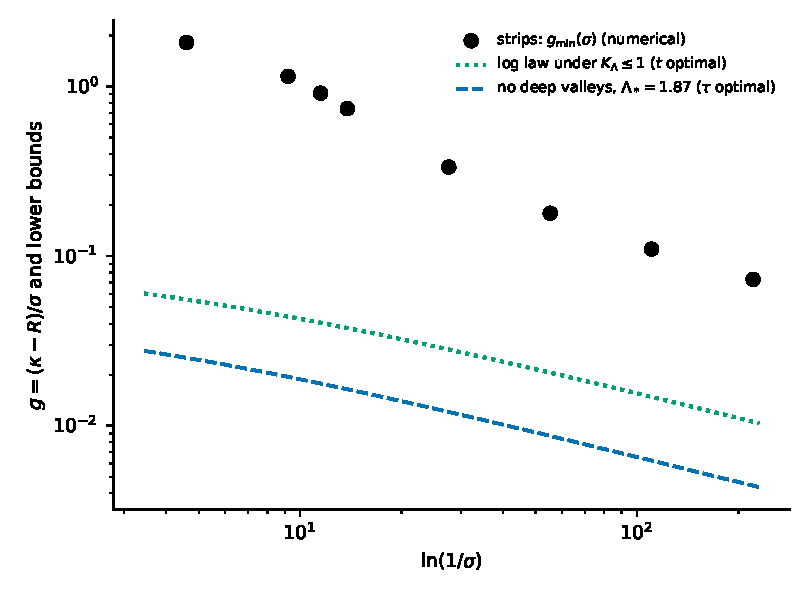
\includegraphics[width=\columnwidth]{figures/fig3_staircase.pdf}
\caption{Lower bounds on $g = (\kappa - R)/\sigma$ against the strips' numerical minimum $g_{\min}(\sigma)$ (dots), with the prefactor $\Pi$ set to one. Dotted: Theorem~\ref{thm:log} with $K_1 = 1$, which covers the strips, and $t$ chosen optimally at each $\sigma$. Dashed: Proposition~\ref{prop:novalley} with the strips' $\Lambda_* = 1.87$, which needs no ratio condition. Both decrease like $1/\sqrt{\ln(1/\sigma)}$, as the strips do.}
\label{fig:staircase}
\end{figure}

\subsection{The ratio $K_\Lambda$}

The ratio $K_\Lambda$ is checkable state by state, and it was small on every family with a small gap: $0.46$--$0.99$ on the strips, $0.69$--$0.78$ on localised ripples, $0.5$ on two clusters, $0.64$ on the hourglass mixture of Ref.~\cite{namba2026gap}, and at most $0.68$ over 36 adversarial maximisations restricted to states with $\sqrt{P_w} \leq 1$. It has, however, no universal bound. For a product state $\rho_1(v)\rho_2(w)$ one finds exactly $K_\Lambda = J_v\|\varrho_v\|^2/(4\|\varrho_v'\|^2)$, where $\varrho_v$ is the blurred first factor and $J_v$ its Fisher information. A wide factor plus a narrow bump of low density gives $K_\Lambda = 0.7$, $1.7$, $5.3$, $23$ and $43$ at $\sigma = 10^{-2}, \dots, 10^{-12}$. These states have large gaps ($\sqrt{P_w}$ between $2.2$ and $10^6$), so they are not counterexamples to the logarithmic law. They show a limit of the proof: $\sqrt\varrho$ sees fine structure in regions of low density that $\varrho$ hardly sees, while such structure cannot support the sharpness near the top that a small gap needs. Section~\ref{sec:removing} removes the ratio condition for broad classes of states by a different route.
